% TODO: Maybe in the \caption[], don't use a final period at the end within the square brackets? Check TOC.
% Great animation about protons going through the CERN accelerator complex.
% https://www.youtube.com/watch?v=FLrEghnKncA

\chapter{THE LARGE HADRON COLLIDER}
\label{ch:lhc}

% OUTLINE
% \section{Motivation for a Large Hadron Collider}
\section{Motivation}
Although the SM
% TODO:(Chapter~\ref{ch:theory})
has shown to be an astoundingly accurate framework so far, it must continue to be scrutinized by the barrage of measurements that either confirm or contradict its predictions.
% cross-examined
Interestingly, a recent measurement of the mass of the \PW boson has shown significant deviation from SM predictions, with a sensitivity of 7$\sigma$~\cite{cdf_collaboration_high-precision_2022}.
After all, undeniable fact comes from reproducible results obtained from measurement---not from some theoretical model which \emph{may} or \emph{may not} describe reality.
Whenever results from measurement contradict the predictions made by a model, the model must necessarily be cast aside and replaced by one whose predictions are in alignment with truth, \ie \emph{measurement}.
% the truth of Nature

So how \emph{are} measurements obtained in the realm of particle physics?
% be continuously tested for its accuracy.
% Must be shaken by the results of experiment to see if its foundation is stable.
% So far, it has upheld against the onslaught of measurements but must be continuously tested for accuracy.
% , it does not explain many phenomena observed in the universe, as discussed in ().
% Although the SM (Chapter~\ref{ch:theory}) is an astoundingly accurate framework, it does not explain many phenomena observed in the universe, as discussed in ().
% As discussed in TODO:PROBLEMS WITH SM, there is observed physics that has not yet been explained in a coherent theoretical and mathematical framework.
% There are currently many searches for physics \emph{beyond the standard model} (BSM) which may explain certain observed physical phenomena that .
% robust, elegant, and accurate (so far), 
% perhaps there is physics beyond the SM (BSM).
% After all, the truth of Nature comes from the results of measurements---not from mathematical and theoretical models.
% Although the standard model (SM) of particle physics  is rather elegant
% and  for the physical phenomena that it does explain.
Modern day physicists study the fundamental constituents of matter and their interactions by using state-of-the-art technologies combined with time-tested methodologies:
%  is to do it the same way humans have been doing it for centuries:
by smashing tiny bits of matter together to turn them into even \emph{tinier} bits.
Such is the purpose of the world's largest and most powerful particle accelerator---the Large Hadron Collider (LHC).
% CERN on a map.
%%%%%%%%%%%%%%%%%%%%
\begin{multiFigure}
    \centering
    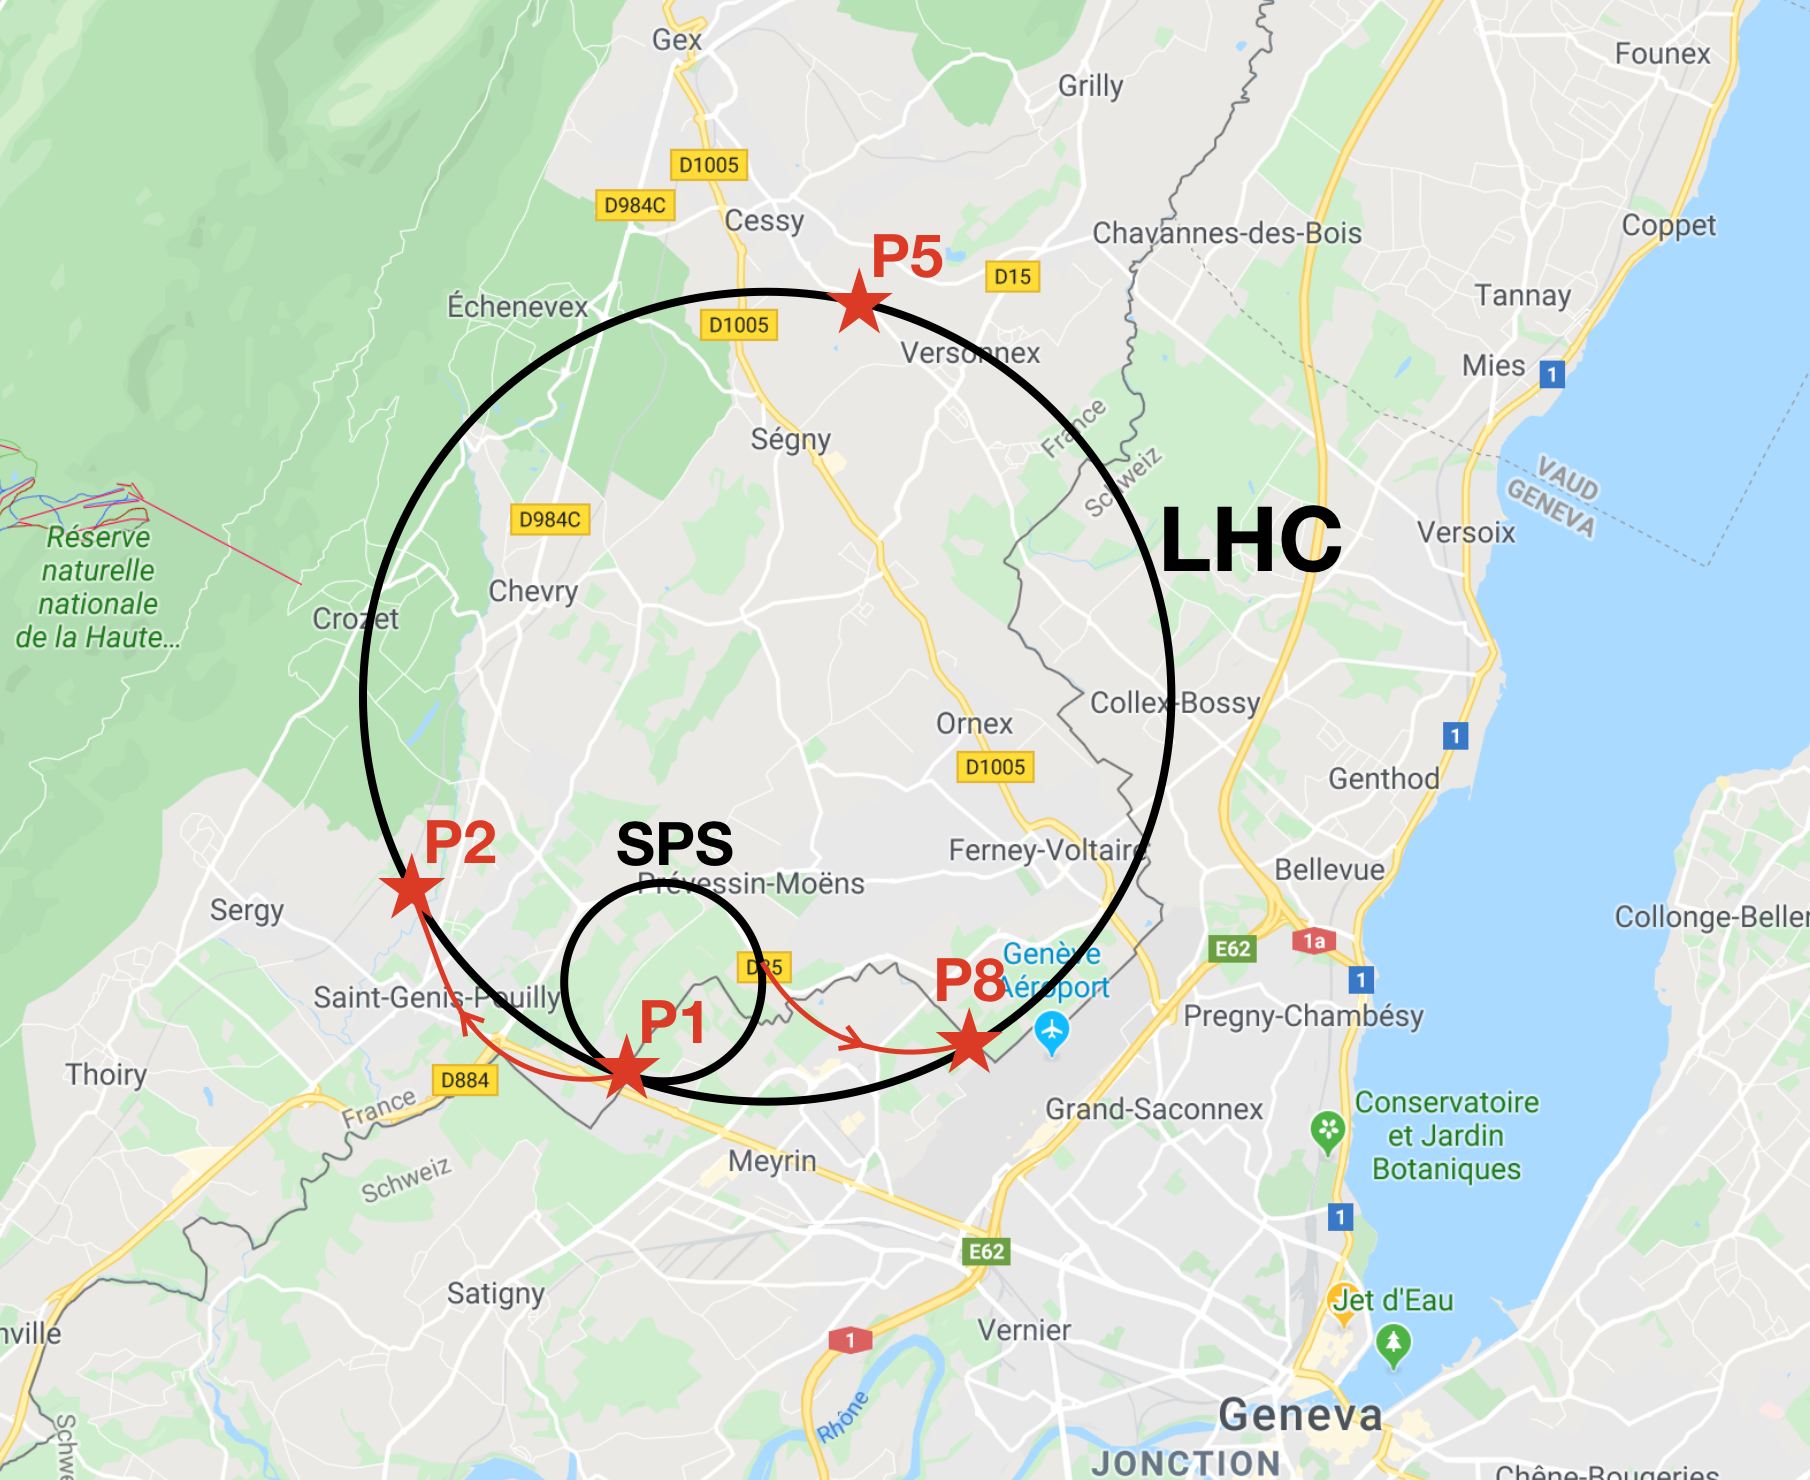
\includegraphics[height=8cm]{figures/lhc/lhc_drawn_on_map_withpoints.png}
    \captionof{figure}
        [The LHC ring superimposed on a map]
        {The LHC (bigger black ring) and Super Proton Synchrotron (SPS, smaller black ring) are drawn to scale, with the neighboring town of Geneva (bottom-right) for size comparison. 
        The four red stars indicate the \pp collision points along the LHC. 
        }
    \label{fig:lhc_on_map}
\end{multiFigure}
%%%%%%%%%%%%%%%%%%%%

\section{The LHC at CERN}
% The circular LHC ring straddles the Franco-Swiss border, approximately 100\meter below the surface of the earth
% (Fig.~\ref{fig:lhc_and_boosters}, Left).
% The ring itself has a circumference of 26.7\Km, making its inscribed area (56.7$\Km^{2}$) almost four times greater than the area of the neighboring city of Geneva (15.9$\Km^{2}$).
% This machine is not only a particle accelerator but also a proton--proton (\pp) collider, sending one beam of protons travelling clockwise and the other beam counterclockwise around the ring. 
Deep beneath the surface of the earth (50--175\meter), the LHC straddles the border shared by France and Switzerland.
Sandwiched between the scenic Jura mountains to the northwest and the sprawling city of Geneva (French: Genève) to the southeast is CERN.
To illustrate the enormous circumference (26.659\Km) of this circular accelerator, Fig.~\ref{fig:lhc_on_map} shows the LHC superimposed to scale on a map.
For reference, the inscribed area of the LHC (56.7$\Km^{2}$) is almost four times greater than the area of the neighboring city of Geneva (15.9$\Km^{2}$).

The LHC is not only a particle \emph{accelerator} but also a proton--proton (\pp), proton--lead ion, and lead--lead ion \emph{collider}.
By sending one particle beam clockwise around the ring and the other beam counterclockwise, the charged particles are carefully maneuvered using dipole magnets and tightly collimated using quadrupole magnets before they ultimately collide at 4 specific points along the LHC, as shown in Fig.~\ref{fig:lhc_on_map}.
% , anywhere from , , and sandwiched between the scenic Jura mountains to the west and the sprawling city of Geneva (Genève) to the east
%  straddles the Franco-Swiss border, approximately 100\meter below the surface of the earth (Fig.~\ref{fig:lhc_and_boosters}, Left).
When the LHC is fully powered, \emph{each} proton in the beam carries an average energy of 6.5\TeV which gives a single \pp collision a massive center-of-mass energy of 13\TeV\footnote{
    For comparison, a \emph{mosquito} in flight carries about 13\TeV of kinetic energy.
    For two \emph{fundamental particles} to collide with this much energy is truly astonishing!
}.
This emulates the conditions theorized to exist at the beginning of the universe, which allows cosmological studies to be carried out.
The hugely energetic \pp collisions cause the quark and gluon constituents within the protons to interact with each other and transform into new particles.
The newly created particles and the residual particle debris are ejected away from the collision point---whether straight down the beampipe, completely orthogonal to it, or somewhere in between.
Massive particle detectors are stationed at each of the 4 collision points to detect the outgoing particle ``spray''.
The 4 main particle detectors and their locations along the LHC are:
\begin{itemize}
    \item A Toroidal LHC ApparatuS (ATLAS)---located at the first collision point, ``P1''
    \item A Large Ion Collider Experiment (ALICE)---located at P2
    \item the Compact Muon Solenoid (CMS, Chapter~\ref{ch:cms}) experiment---located at P5
    \item the LHC-beauty (LHCb) experiment---located at P8
\end{itemize}
% TODO: Get rid of extra newline that appears after itemize.
% ATLAS	A Toroidal LHC Apparatus
% CMS	Compact Muon Solenoid
% LHCb	LHC-beauty
% ALICE	A Large Ion Collider Experiment
% TOTEM	Total Cross Section, Elastic Scattering and Diffraction Dissociation
% LHCf	LHC-forward
% MoEDAL	Monopole and Exotics Detector At the LHC
% FASER	ForwArd Search ExpeRiment
% SND	Scattering and Neutrino Detector

The world-renowned feat of digging the tunnel for, constructing, commissioning, and monitoring the LHC was made possible by CERN:
% - Before the LHC, LEP was originally in the tunnel.
%     - LEP ran from TODO--TODO.
the European Organization for Nuclear Research (French: \emph{Conseil Européean pour la Recherche Nucléaire}).
CERN is an international collaboration of---at the time of this writing---more than 33 countries,
% it's actually 34.
% Learn about the series of accelerators here:
% https://cdsweb.cern.ch/record/2771424/files/CERNAnnualReport_2020_EN.pdf
each of which is considered either a Member State, an Associate Member State, or an Observer.
The complex of CERN (Fig.~\ref{fig:lhc_complex}) is located just to the west of P1 and is akin to a small science \emph{city}---complete with many offices, manufacturing facilities, and experiments such as the Antiproton Decelerator (AD), the Neutrons Time of Flight (n$\_$TOF), and the Isotope Separator OnLine (ISOLDE) experiments.
% the world's largest and most powerful particle accelerator, the Large Hadron Collider (LHC).
% The completion of this world-renowned feat was only possible through the careful efforts of thousands of scientists, engineers, administrators, \etc from all over the world.
% At the time of this writing, CERN is associated with at least 33 countries, each of which is considered either a Member State, an Associate Member State, or an Observer.
Although the LHC is the most famous of the accelerators at CERN, its fame is only made possible by a series of smaller and lesser-known accelerators that \emph{feed} the LHC.
% would not be able to accelerate \emph{any} charged particles from rest; not collide particles at such massive energies if not for the lesser-known accelerators that feed into the LHC.
% but it takes clever engineering and a series of smaller accelerators to eventually feed particles into the LHC to reach their maximum energy of 6.5\TeV.
Therefore, a natural way to explore the intricacies and inner workings of the LHC is to follow the path of one of its ``inhabitants''---a single proton---as it makes its way to and through the gigantic collider.
% Accelerator complex at CERN.
%%%%%%%%%%%%%%%%%%%%
\begin{multiFigure}
    \centering
    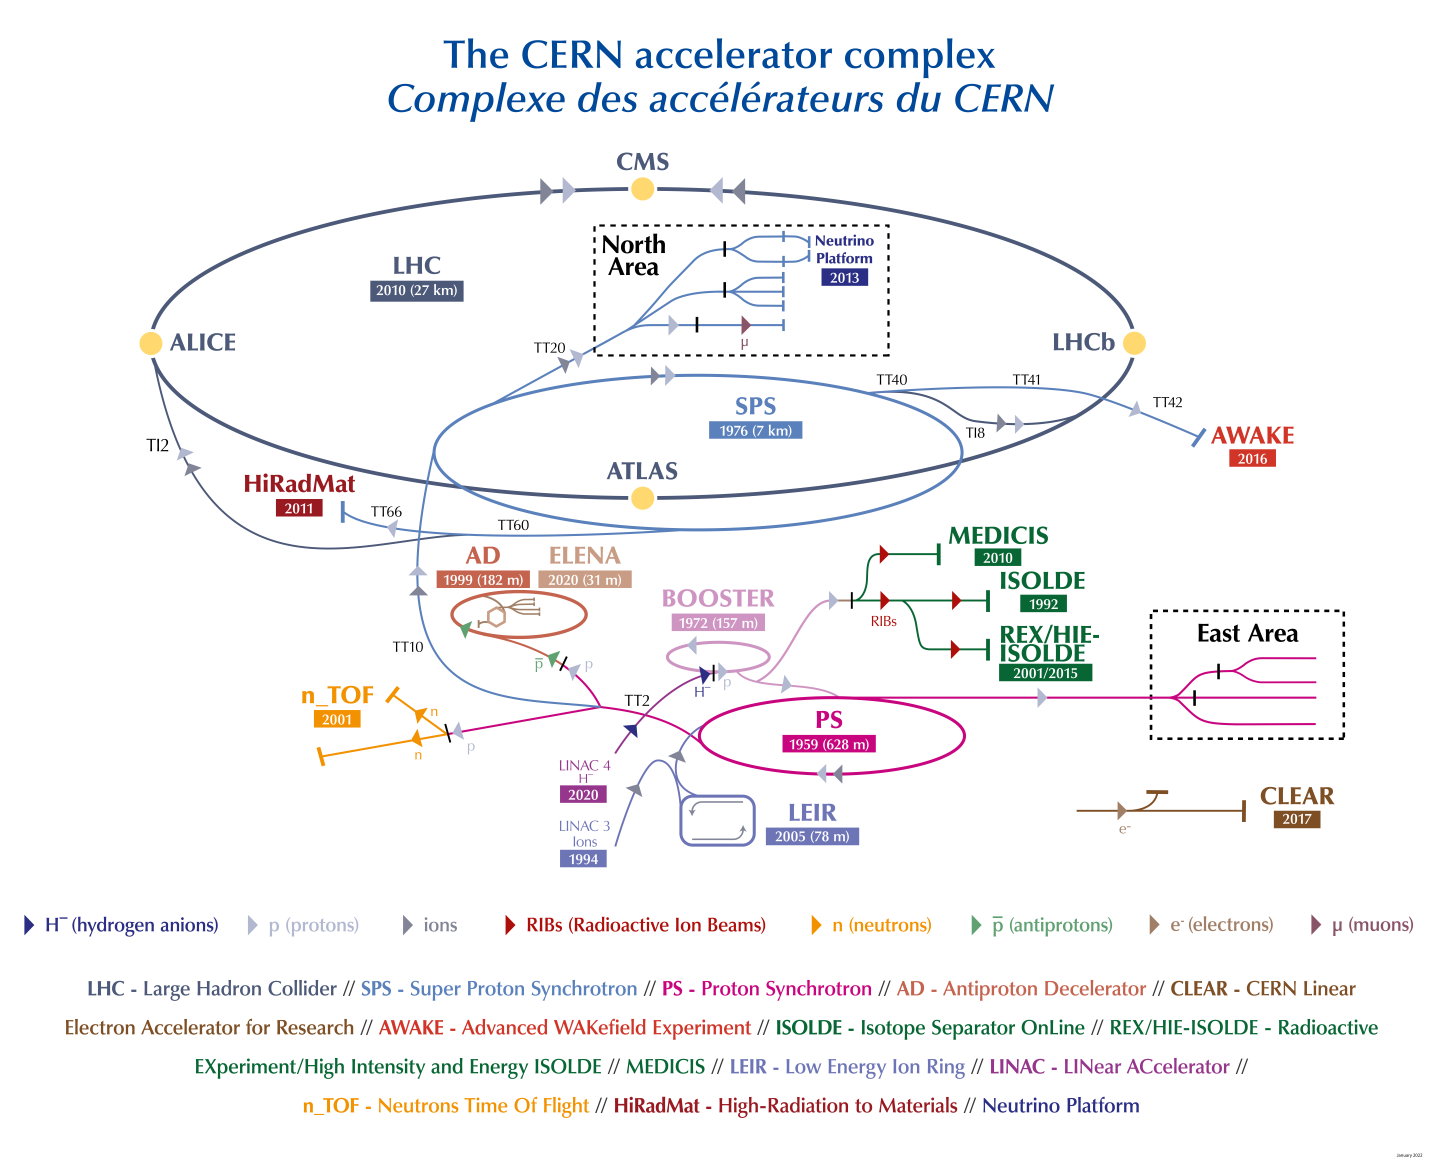
\includegraphics[height=12.5cm]{figures/lhc/cern_complex.png}
    \captionof{figure}
        [The accelerator complex at CERN]
        {The accelerator complex at CERN.}
    \label{fig:lhc_complex}
\end{multiFigure}
%%%%%%%%%%%%%%%%%%%%

\section{The Journey of a Proton at the LHC}
The journey to discovery begins in a surprisingly small tank of hydrogen gas (\htwo) located in the LINAC4 building at the main CERN site.
% , in which a proton that is bound to another proton as a molecule of H2 .
% Pic of hydrogen source from here: https://www.lhc-closer.es/taking_a_closer_look_at_lhc/0.linac4
Inside this tank, a proton---conveniently named Paul Roton, or just \pname for short---and $\mathcal{O}(\tentothe{23})$ other protons (TODO:DOUBLE CHECK THIS)
coexist in bound states as molecules of H$_2$.
Although the tank has a meager mass of 
% TODO: Double check this number.
$\approx$10\Kg,
it has enough protons inside to keep the LHC colliding protons for over \emph{200\,000 years} of constant operation.

\pname and the rest get injected into a series of increasingly larger and more powerful accelerators.
They begin their journey at the \emph{Linac4}---a linear particle accelerator---that converts the particles into hydride ions (H$^-$) and then accelerates them to 160\MeV, at which point, they are fed into the \emph{Proton Synchrotron Booster} (PSB).
In the PSB, each H$^-$ has its electron pair completely stripped away, leaving only the bare proton ($\Pp^+$).
\pname then enters a series of circular accelerators, where each machine feeds its protons into the next in order to increase the proton center-of-mass energy by at least 1 order of magnitude with each feeding.
The flow of accelerators is as follows:
\begin{itemize}
    % TODO: mention electric field?
    % \item The flow 
    \item From the PSB, \pname are the rest are accelerated to 2\GeV and then injected into the \emph{Proton Synchrotron} (PS).
    \item The PS increases the energy of the particles to 26\GeV and then feeds the protons into the \emph{Super Proton Synchrotron} (SPS).
    \item Next, the SPS energizes the protons to a center-of-mass energy of 450\GeV and sends bunches of protons (so-called \emph{proton bunches}, $\mathcal{O}\left(\tentothe{11}\right)$ protons) into the LHC. %  $\approx$$\tentothe{11}$  are packed together into a ``proton bunch''. % a accelerates protons to com energy
\end{itemize}
% TODO: Mention: A single proton bunch is about the size of a human hair ($\approx$50\mum wide and $\approx$10\cm long). 
% TODO: Mention: The clockwise and counterclockwise rings are filled to a maximum of 2808 proton bunches, each one spaced 25\ns apart, and then sent to collide. 
It is inside the LHC that \pname and its fellow protons within its proton bunch are given precisely timed \emph{kicks} by the electric field\footnote{
    The electric field quickly oscillates between pointing parallel to the direction of travel of the proton bunch to pointing \emph{antiparallel} to the direction of travel.
    Therefore, precise timing is required to ensure that the electric field only points parallel so as to speed up the protons in the proton bunch.
    This is analgous to the timing required when pushing a person on a swing:
    the pusher must push at \emph{just} the right time to increase the momentum of the one swinging, lest the pusher slows the swinger down!
} within radio-frequency (RF) cavities.
After sufficient energy is delivered to the proton bunches, they finally achieve their max speed of 0.999\,999\,990$c$ (corresponding to a Lorentz factor of $\gamma \approx 7000$). %  Wikipedia says 6930.  99.999\,996\%$c$.
At this speed, \emph{each proton} in the proton bunch carries a center-of-mass energy of 6.5\TeV.

\pname and its neighboring protons in the proton bunch are nearly ready for a head-on collision with another proton bunch to make interesting physics.
The only problem is that the proton bunches must be turned (to keep them in the circular LHC) and must be tightly squeezed down (to increase the chance of \pp collisions).
Since the protons are bare, they are all positively charged, and are subject to a Lorentz force when they pass through a magnetic field.
Therefore, the LHC is equipped with 1232 dipole magnets distributed all along its circumference to turn the proton bunches.
The cross section of such a dipole magnet is shown in Fig.~\ref{fig:lhc_dipole_xs}.
Each dipole magnet is 14.3\meter long, weighs 35\tonne, costs nearly 500\,KCHF to produce, and has nearly 11\,700\,A of current running through it.  % TODO: make command for amps unit?
Only with such massive currents is it possible to generate the necessary magnetic field strength of 8\tesla to keep the protons moving in a circular fashion at their near-light speed. 
The magnetic field is maintained by copper-clad niobium-titanium coils, which requires the cryogenics conditions of 96\tonne of superfluid helium-4 to achieve the necessary temperature of 1.9\kelvin to reach a superconducting state; 
this temperature is colder than that of outer space.
% TODO: Check numbers here and ref.
There are also 506 quadrupole magnets (TODO:CITE) that compress the proton bunches as tightly as possible before collision with the other oncoming proton beam.
%%%%%%%%%%%%%%%%%%%%
\begin{multiFigure}
\centering
    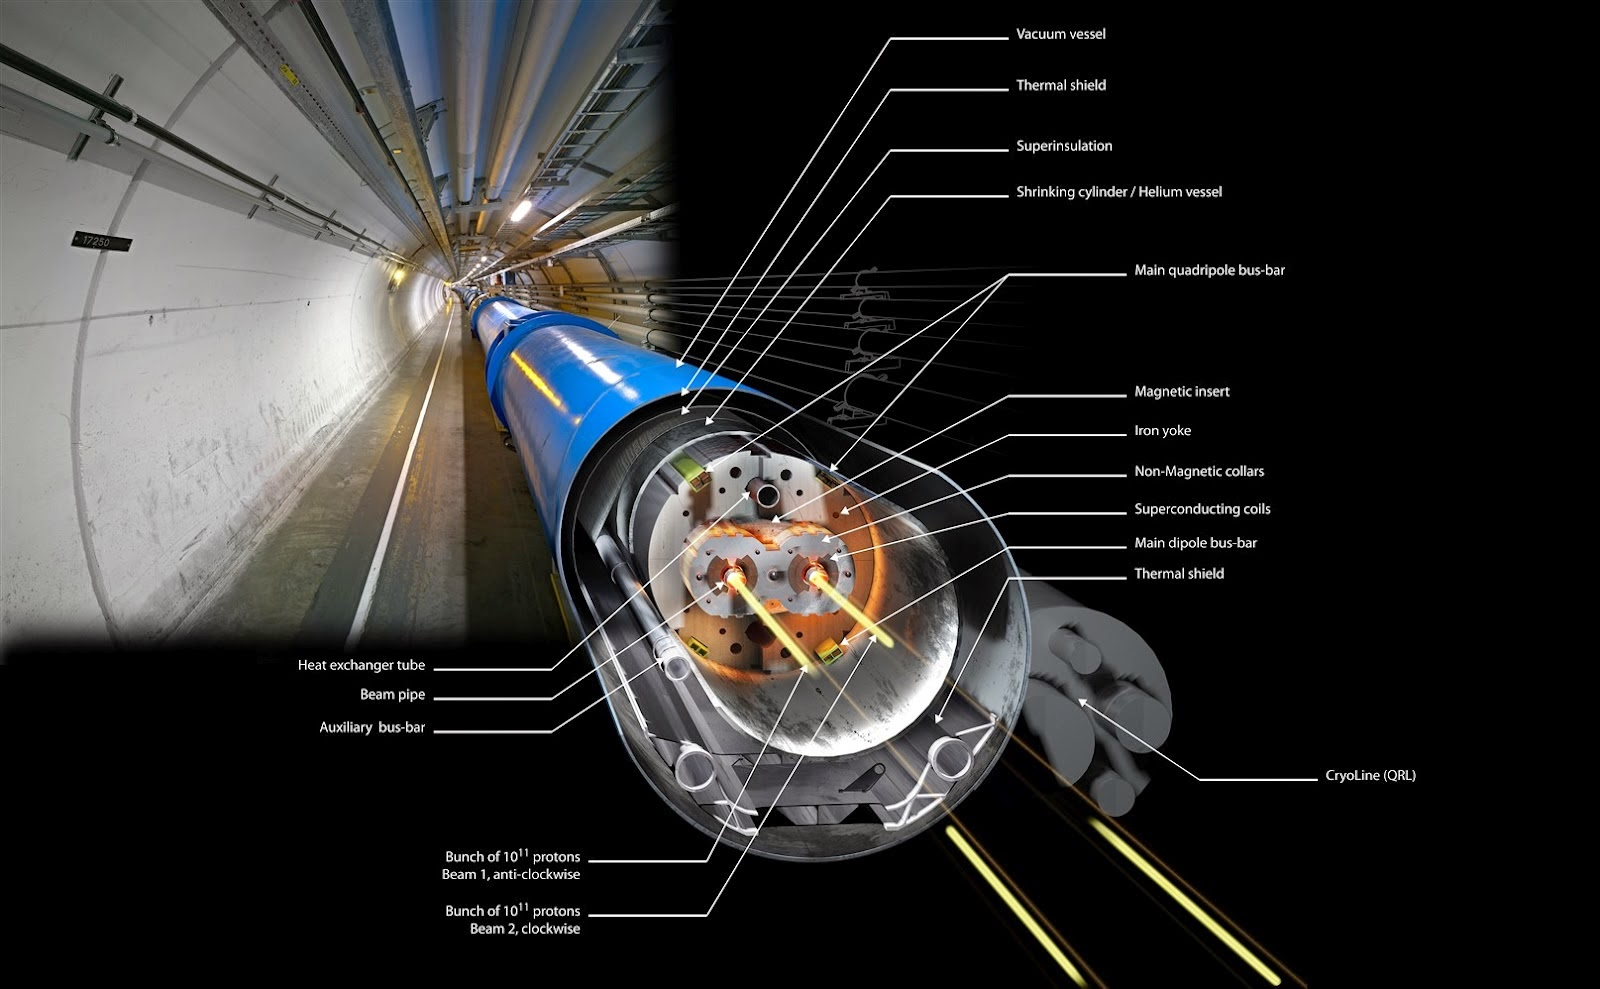
\includegraphics[height=10cm,keepaspectratio]{figures/lhc/lhc_dipole_xs.jpg}
    \captionof{figure}
        [Cross section of a dipole magnet at the LHC]
        {A cross section of one of the 1232 dipole magnets which span the entire length of the LHC tunnel.} 
    \label{fig:lhc_dipole_xs}
\end{multiFigure}
%%%%%%%%%%%%%%%%%%%%

% As two bunches (one from the clockwise proton beam and the other from the counterclockwise beam) approach one of the four detector points along the LHC, each bunch is squeezed tightly using quadrupole magnets, helping to focus the beams which increases the chance for the desired \pp collisions.
As the two proton beams approach one of the four detector points along the LHC, two of the oncoming bunches are squeezed tightly using the quadrupole magnets which increases the chance for the desired \pp collisions.
During a bunch crossing (BX), amazingly most of the protons just pass right by one another; 
out of the $\approx$$\tentothe{11}$ possible \pp collisions that could have occurred, Fig.~\ref{plt:pileup} shows that on average only approximately 32 collisions occurred per BX during the 2018 Run of the LHC. %, according to a particle detector called CMS, described in Chapter~\ref{ch:cms}.  a mere 50 collisions take place on average (\ie only 0.0001\%).
This is a testament to just how small protons truly are.
%%%%%%%%%%%%%%%%%%%%
\begin{multiFigure}
    \centering
    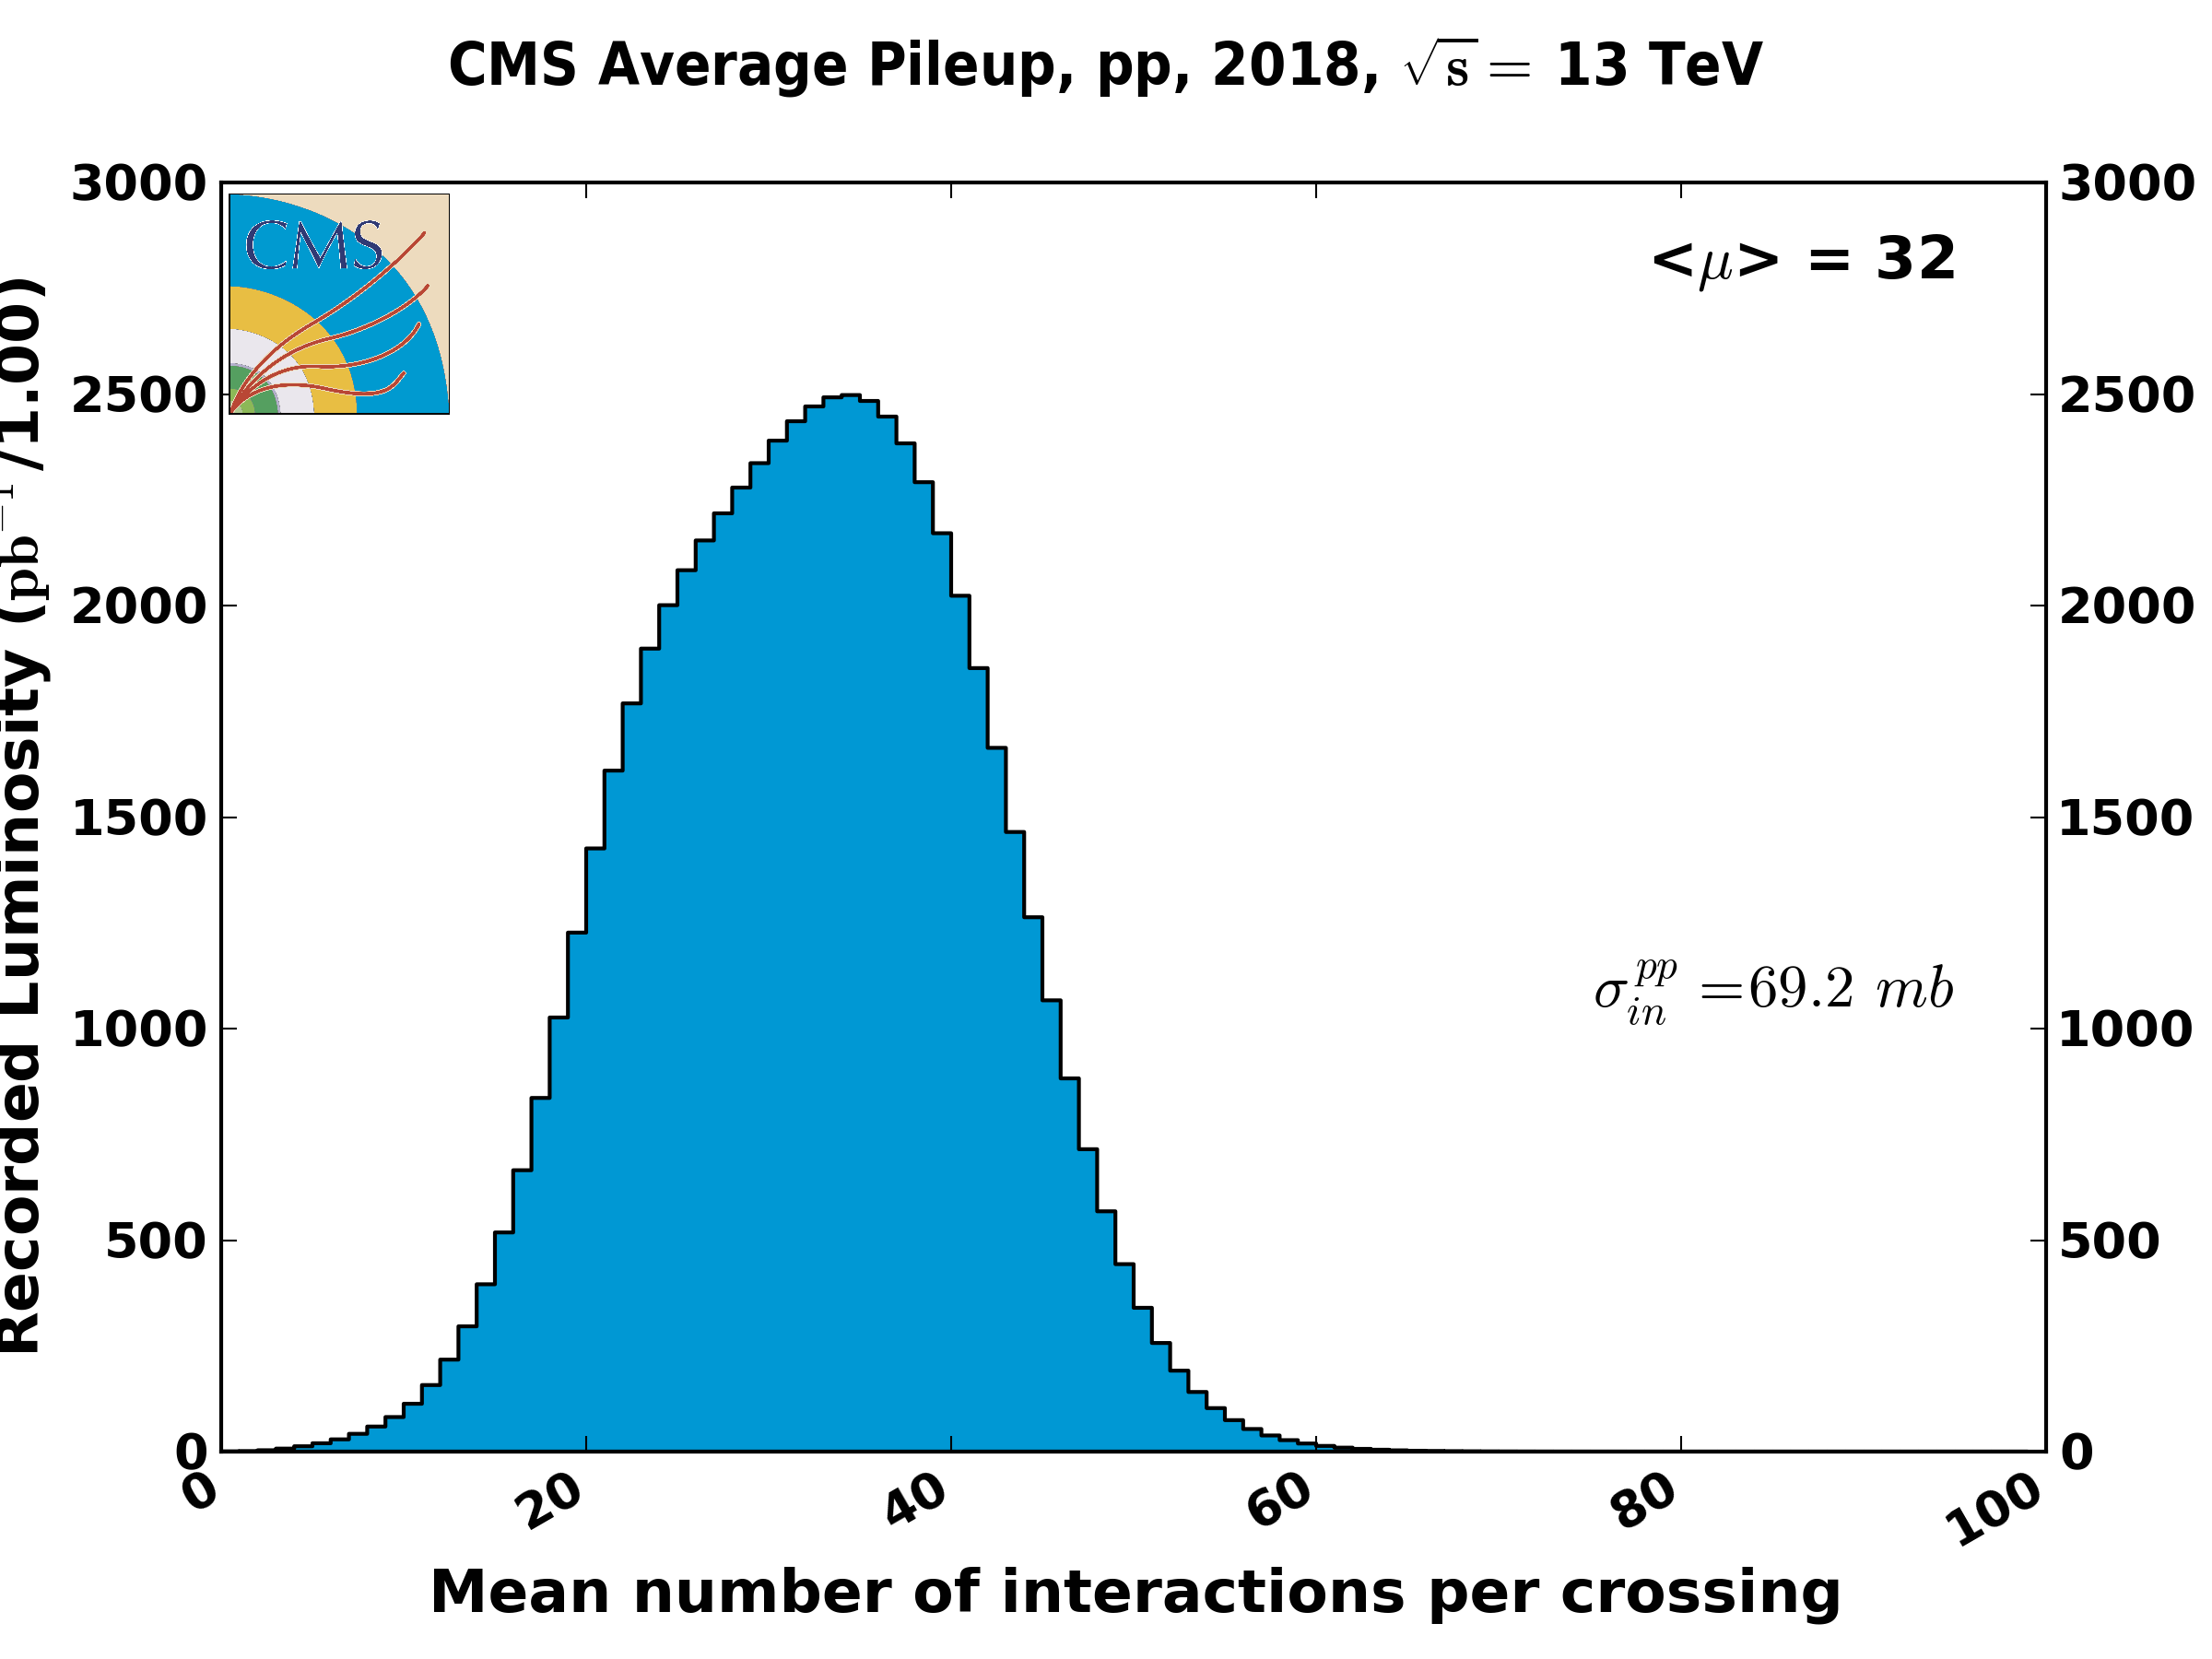
\includegraphics[width=0.7\textwidth,keepaspectratio]{figures/lhc/pileup_pp_2018.png}
    \captionof{figure}
        [Average pileup distribution during the LHC 2018 run]
        {Distribution of the average number of \pp collisions per proton bunch crossing (\emph{pileup}) which CMS recorded during the LHC 2018 run.} 
    \label{plt:pileup}
\end{multiFigure}
%%%%%%%%%%%%%%%%%%%%

%from 50 $\mu$m
In the event that \pname does not collide with any of the oncoming protons, then it is simply ``recycled'' and continues going around the LHC ring for another opportunity at a \pp collision.
When the anticipated moment finally comes---\ie a ``hard'' \pp collision is realized, as shown in Fig.~\ref{fig:pp_collision}---the energy of the single collision contains a monstrous center-of-mass energy of \sqrtsthirteen, which is more than enough to create new particles like top quarks, Higgs bosons (Chapter~\ref{ch:higgs_mass}), and potentially BSM particles (Chapter~\ref{ch:dilep_res}).
% Truly, it is the particles inside the protons, the so-called \emph{partons} that interact with one another, as shown in Fig.~\ref{fig:pp_collision}.
In order to analyze such interesting particles, one needs to detect the outgoing particles produced from the \pp collisions.
One such dedicated particle detector is located at Point 5---the Compact Muon Solenoid (CMS) detector---and is described in the next chapter.
%%%%%%%%%%%%%%%%%%%%
\begin{multiFigure}
    \centering
    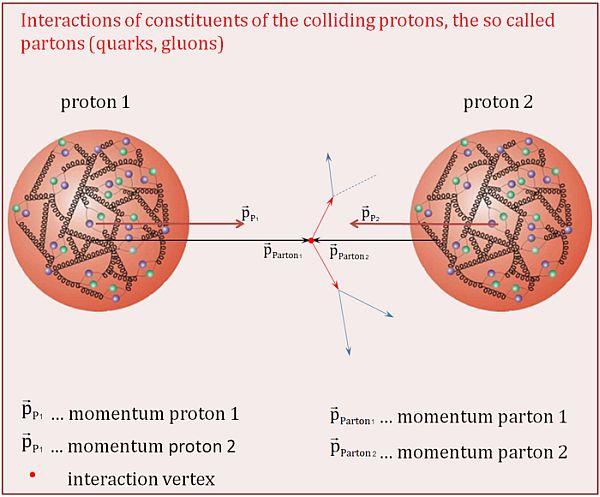
\includegraphics[width=0.8\textwidth]{figures/lhc/proton_proton_quarksandgluons.jpg}
    \captionof{figure}
        [Diagram showing the constituent (\emph{partons}) of two protons interacting in a \pp collision]
        {Two protons can be smashed together at very high energies at the LHC $\left( \sqrtsthirteen \right)$ to have their constituent partons interact and convert into new kinds of matter.} 
    \label{fig:pp_collision}
\end{multiFigure}
%%%%%%%%%%%%%%%%%%%%

% Finally two incoming proton bunches approach a common collision point.
% - Frequency of BX: considering that proton bunches are spaced 25\ns apart, this means 

% TODO: FCC?
% Just as the PS feeds protons into the SPS, which feeds protons into the LHC, so too is it being considered for the LHC to feed a new project---the 100\Km Future Circular Collider.


% LPS SPS
% into a beam pipe going clockwise and another 2800 bunches going around counterclockwise, 

% TODO:
\section{Physics of the LHC}
The merit of a particle collider is typically judged by its center-of-mass energy and a second parameter: the \emph{luminosity}.
In essence, luminosity refers to the `brightness' of the colliding particle beams,
\ie the more tightly packed the particle bunches are, the higher the number of particles per bunch, the more frequently the bunches collide, then the higher the luminosity will be.
Concretely, the instantaneous time-dependent luminosity $(\lumi(t))$ is defined as the ratio between the expected rate $\left( R(t) \right)$ of events and the corresponding cross section $(\sigma)$ for some physics process:
\begin{equation}
    \lumi(t)= \frac{R(t)}{\sigma}.
    \label{eqn:lumi_def}
\end{equation}
Physicists are interested in the total number of events $\left( N^\text{exp} \right)$ they should expect to see in the laboratory---observing a number of events significantly different enough from $N^\text{exp}$ may hint at new physics.
Rearrangement of Eqn.~\ref{eqn:lumi_def} and setting $R(t) = \text{d}N^\text{exp} / \dt$ gives the infinitesimal change in the number of expected events after a small increment of time $(\dt)$:
\begin{equation}
    \frac{\text{d}N^\text{exp}}{\dt} = \sigma \lumi(t).
    \label{eqn:dNdt}
\end{equation}
Collider experiments typically last over long time periods, so integrating Eqn.~\ref{eqn:dNdt} from some starting time $\left( t_1 \right)$ to some later time $\left( t_2 \right)$, gives $N^\text{exp}$:
\begin{align*}
    N^\text{exp} &= \sigma \int_{t_1}^{t_2}{\lumi(t) \dt}
    \\
    \implies N^\text{exp} &= \sigma \lumiint,
    \label{eqn:Nexp}
\end{align*}
where $\int_{t_1}^{t_2}{\lumi(t) \dt} \equiv \lumiint$ and $\sigma$ is assumed to be independent of time.
% The term $\int_{t_1}^{t_2}{\lumi(t) \dt}$ is the aptly named \emph{integrated luminosity} $\left( \lumiint \right)$ and is a measure of the amount of data collected from $t_1$ to $t_2$.
The term \lumiint is aptly named \emph{integrated luminosity} and is a measure of the amount of data collected from $t_1$ to $t_2$.

When two proton bunches cross at the LHC, the instantaneous luminosity $\left( \lumi_\text{b}\right)$ can be calculated using the so-called \emph{van der Meer method}~\cite{LUM-17-003}:
\begin{equation}
    \lumi_\text{b} = \frac{f_r  n_1  n_2}{A_\text{eff}},
    \label{eqn:lumi}
\end{equation}
where $f_r$ is the LHC frequency of revolution of the particle bunches (11\,245.6\Hz) during collisions,
$n_1$ and $n_2$ are the numbers of particles in each bunch,
and $A_\text{eff}$ is the effective area of overlap between the two bunches.
Since the particle bunches are not infinitely narrow but instead have a cross-sectional profile, $A_\text{eff}$ can be put into terms of the widths of each bunch.
Specifically, if the bunches collide head-on, are Gaussian-distributed, and have the same root-mean-square beam widths ($\sigma_x$ and $\sigma_y$, in the $x$ and $y$ directions, respectively), then Eqn.~\ref{eqn:lumi} becomes:
\begin{equation}
    \lumi_\text{b} = \frac{f_r  n_1  n_2}{4\pi \sigma_x \sigma_y}.
    \label{eqn:lumi_final}
\end{equation}

From Eqn.~\ref{eqn:lumi_final}, it is easy to validate the intuitive description of luminosity as described at the beginning of this section:
$\lumi_\text{b}$ is directly proportional to the numbers of particles in each bunch and to the frequency of revolution,
and it is inversely proportional to the beam widths.
% TODO: Include the below?
% Using the values of the LHC ($f_r = 11\,245.6\Hz$, ) This yields 


% The luminosity of the LHC is $\mathcal{O}(\LHigh)$ the number of particles 
% It should be mentioned that the luminosity of the LHC is on the order of \LHigh. %$10^{34}$ Hz/cm$^2$.

% SPECS
% - Luminosity
% - rates
% - data

% N obs events = xs * eff * Lint 
% cross section is specific to the process
% efficiency is ideally unity.




% The LHC has ushered in the era of ``TeV-scale physics'',
% exploring the 
% - which is about the same amount of energy of a really fat flying mosquito.

% It takes a proton \~90 $\mu$s 
% to make a complete revolution around the LHC moving at such a speed.

% Higgs boson produced every 1 billion collisions.

% Beginning in 2026 (FIXME), the LHC will undergo a ``Phase 2'' upgrade and become the High-Luminosity LHC.
% This upgrade will increase the collider's luminosity by 10 fold (FIXME) and is predicted to deliver SO much data 3000 fb?.

% TODO:
% \section{High-Luminosity LHC}
